% The Figure 1 schematic. Exported to ../figure.png for the README; the same
% tikzpicture is pasted inline in the report, so the two cannot drift as long as
% this file is the thing that gets edited.
%
%   pdflatex schematic.tex
%   magick -density 300 schematic.pdf -quality 95 ../figure.png
%
\documentclass[tikz,border=4pt]{standalone}
\usepackage{tikz}
\usepackage{xcolor}

\definecolor{wongblue}{RGB}{0, 114, 178}
\definecolor{wongorange}{RGB}{230, 159, 0}
\definecolor{wonggrey}{RGB}{100, 100, 100}

\begin{document}
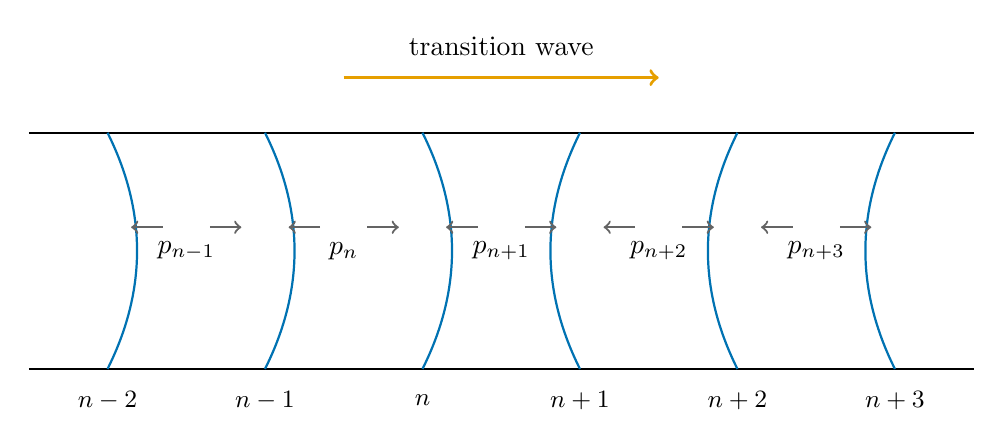
\begin{tikzpicture}[scale=1]
    % pipe walls
    \draw[thick] (0, 1.5) -- (12, 1.5);
    \draw[thick] (0, -1.5) -- (12, -1.5);

    % switched diaphragms behind the wave: bent right
    \draw[thick, wongblue] (1, -1.5) .. controls (1.5, -0.5) and (1.5, 0.5) .. (1, 1.5);
    \draw[thick, wongblue] (3, -1.5) .. controls (3.5, -0.5) and (3.5, 0.5) .. (3, 1.5);
    \draw[thick, wongblue] (5, -1.5) .. controls (5.5, -0.5) and (5.5, 0.5) .. (5, 1.5);

    % unswitched diaphragms ahead of the wave: bent left
    \draw[thick, wongblue] (7, -1.5) .. controls (6.5, -0.5) and (6.5, 0.5) .. (7, 1.5);
    \draw[thick, wongblue] (9, -1.5) .. controls (8.5, -0.5) and (8.5, 0.5) .. (9, 1.5);
    \draw[thick, wongblue] (11, -1.5) .. controls (10.5, -0.5) and (10.5, 0.5) .. (11, 1.5);

    % diaphragm labels
    \node at (1, -1.9) {\small $n-2$};
    \node at (3, -1.9) {\small $n-1$};
    \node at (5, -1.9) {\small $n$};
    \node at (7, -1.9) {\small $n+1$};
    \node at (9, -1.9) {\small $n+2$};
    \node at (11, -1.9) {\small $n+3$};

    % pocket pressures, arrows pushing on both bounding diaphragms
    \node at (2, 0) {$p_{n-1}$};
    \draw[->, thick, wonggrey] (1.7, 0.3) -- (1.3, 0.3);
    \draw[->, thick, wonggrey] (2.3, 0.3) -- (2.7, 0.3);

    \node at (4, 0) {$p_n$};
    \draw[->, thick, wonggrey] (3.7, 0.3) -- (3.3, 0.3);
    \draw[->, thick, wonggrey] (4.3, 0.3) -- (4.7, 0.3);

    \node at (6, 0) {$p_{n+1}$};
    \draw[->, thick, wonggrey] (5.7, 0.3) -- (5.3, 0.3);
    \draw[->, thick, wonggrey] (6.3, 0.3) -- (6.7, 0.3);

    \node at (8, 0) {$p_{n+2}$};
    \draw[->, thick, wonggrey] (7.7, 0.3) -- (7.3, 0.3);
    \draw[->, thick, wonggrey] (8.3, 0.3) -- (8.7, 0.3);

    \node at (10, 0) {$p_{n+3}$};
    \draw[->, thick, wonggrey] (9.7, 0.3) -- (9.3, 0.3);
    \draw[->, thick, wonggrey] (10.3, 0.3) -- (10.7, 0.3);

    % direction of travel
    \draw[->, very thick, wongorange] (4, 2.2) -- (8, 2.2);
    \node at (6, 2.6) {transition wave};
\end{tikzpicture}
\end{document}
